\section{Analysis of results}\label{sec:analysis-of-results}
This section presents an interpretation of data from the evaluations.

\todo[inline]{probably i'll have to describe the languages better if i want to draw some conclusions here}

\subsection{Architecture and structure)}\label{subsec:4-2-architecture-and-structure}
Support for architectural concepts in the representations was varied: some of them support more concepts (Gaouar, XANUI, OpenUIDL) and some \textendash\ less (Khan, Soude, Quid).
This might have been caused by different goals that these representations have.
For example, Quid is a minimal language and a browser tool for prototyping Web components \textendash\ it is therefore understandable that it does not support modelling full applications.
That is, however, what OpenUIDL is intended for, therefore it can make use of these concepts.

As was exemplified by the case of Quid, not all representations use the concept of an application/project (\textbf{A1}).
Dialogs (\textbf{A3})and third-party components (\textbf{A6}) were not also widely supported \textendash\ the former was only supported by a single representation (Verhaeghe), and the latter \textendash\ by two (OpenUIDL, XANUI).

\subsection{Logic and behavior}\label{subsec:4-2-logic-and-behavior}
Support for specifying the behavior of UI in the representations was also varied, but in general rather low \textendash\ only two representations scored over 50\% (Soude, XANUI) with the maximum score of around 66\%;
\todo{include this phrase?}the level of support varied from area to area
Most representations indeed allow for handling events and attaching methods to UI elements (\textbf{B1});
however, only a few allow for actually defining handlers (\textbf{B3}) that could perform any actions, either in a broad way (\textbf{B4}), or in detail (B8.1, \textbf{B8}, \textbf{B10}, \textbf{B10}, \textbf{B11}).
Sets of predefined events (\textbf{B2}) also varied in their scope from minimal (XANUI, Soude, Quid, Gaouar) to comprehensive (Verhaeghe, OpenUIDL).

Only one representation (XANUI) explicitly supported data validation (\textbf{B5}).
More were able to integrate with code outside of the UI layer, either by calling some services (\textbf{B6}) or directly embedding scripts (\textbf{B7}).

Support for custom components (\textbf{B12}) was relatively rare \textendash\ only three representations meaningfully implemented this feature (XANUI, OpenUIDL, Quid).
Especially rare was support for content as input (supported by Quid) and real component methods (provided in Quid).

Khan et al.\ explicitly stated in their description of the representation that it does not concern behavior which needs to be implemented manually.
Although Verhaeghe et al.\ successfully used their description to migrate both the content and the logic of UIs, this success does not seem to translate to modelling on its own.
This might be the case, because their behavior metamodel is based on a model of the abstract syntax tree (AST) of the original code;
\todo{does this make sense?}therefore it does not introduce any new concepts specific to the modelling task.

Quid allows for handling events and even for explicit definition of handlers; its capabilities are nevertheless limited in other areas.
Gaouar also allows for defining handlers; on one hand, it is even possible to call external services, on the other \textendash\ they are rather limited in terms of control structures and operators.
OpenUIDL also has very limited capabilities of specifying behavior, for which it makes up with more comprehensive support for custom components and a wider set of predefined events.

Soude and Koussonda also allow for specifying handlers (at least for input components) and using external (REST) services.
Additionally, they comprehensively support a range of expression operators and data types.
XANUI offers the most capabilities for specifying behavior, as it is an annotation language \textendash\ it is embedded into an original implementation language which allows it to take advantage of its expressiveness.
However, it also provides a few constructions on its own (e.g.\ handlers and data validation).

\subsection{Component support}\label{subsec:4-2-component-support}
Support for predefined components in the chosen representations ranges from low to medium.
The least supported category are complex output components (\textbf{C3})and specialized containers (\textbf{C1}) \textendash\ such a result is relatively understandable, as supporting additional types of components requires effort on the part of maintainers.
Interaction components (\textbf{C6}) and simple output components (\textbf{C2}) are moderately supported;
so are input components (\textbf{C4}), although usually their implementation lacks customization abilities (\textbf{C5}).

There does not seem to be any technical limitation that would explain the more or less limited set of components offered by the representations \textendash\ the results seem to be motivated by a subjective judgement of authors.
To be able to support them, maintainers would need to define them in the model and \todo{i'm feeling a stroke here}define a transformation rule for them to be included in the final code \textendash\ indeed, that is the approach Verhaeghe et al.\ recommend to users of their representation who want to include widgets not foreseen by the original authors.

The only exception to the rule could be XANUI \textendash\ the relative lack of support for predefined components might also be explained \todo{stroke}by its relationship to the final UI code.

\subsection{Appearance}\label{subsec:4-2-appearance}
Support for describing appearance of the final UI is the most varied from all sections: some representations do not incorporate that aspect at all (Soude), while some have surprisingly comprehensive support (OpenUIDL).

Most languages support a linear layout (D1.1), \todo{stroke}as it can cover most of the needs;
some also specify an additional one, like a flex layout (D1.2), or a relative layout (D1.4).
A few languages (Gaouar, Khan, OpenUIDL) support responsive layouts through media queries.

There is very varied support for sizing (\textbf{D3}) and positioning (\textbf{D5}) \textendash\ some representations provide most of all methods, and some none.
Only OpenUIDL provides a relatively wide set of sizing units (\textbf{D4});
most representations limit themselves to pixels (D4.1) and percentages of parent (D4.4).

When it comes to other style properties (\textbf{D6}, \textbf{D7}), support is either rather comprehensive (Khan, OpenUIDL) or nonexistent (Verhaeghe).
Extended capabilities for describing the appearance through CSS are only provided in two representations (Khan, OpenUIDL).

Similarly to support for components, the level of detail in the model of appearance seems to be \todo{stroke}a matter of goal specification and subjective decisions.
Some representations (Quid, Soude) dismiss this area;
others model it with greater or smaller accuracy.
XANUI again does not include too much information about appearance, as this problem might be resolved natively.

The capabilities of OpenUIDL are by far the greatest of all sections; \todo{stroke}it also scores the most in this section from all others.
The representation scored high (\todo{stroke}or complete score) on almost all criteria, with one exception of layout capabilities.
The reason for this might be because the language is mostly \todo{stroke}targeted towards Web applications, where layouts other than linear or flex are not useful.

\subsection{All sections}
My conclusions are:
\begin{itemize}
    \item some languages have good support in some areas, but no language includes everything
    \item none of the languages seem really flexible and productive
    \item Quid is a very simple language, simple support for logic, but no appearance and components
    \item Soude and Koussonda, Khan have some strong and weak areas
    \item XanUI has strong support for logic, but little components and support for appearance \textendash\ however, this might be because it doesn't need to be handled by the language
    \item Verhaeghe and Gaouar have a little bit of everything, but do not excel in any particular area
    \item OpenUIDL is the most expressive, with good architectural support, decent component support and strong customizability of appearance; the only weak area is logic - there aren't many possibilities to define handlers and state and change it
\end{itemize}

Look at the diagrams~\ref{fig:4-2-results-per-section},~\ref{fig:4-2-results-per-representation}, and~\ref{fig:4-2-results-total}:
\begin{figure}
    \centering
    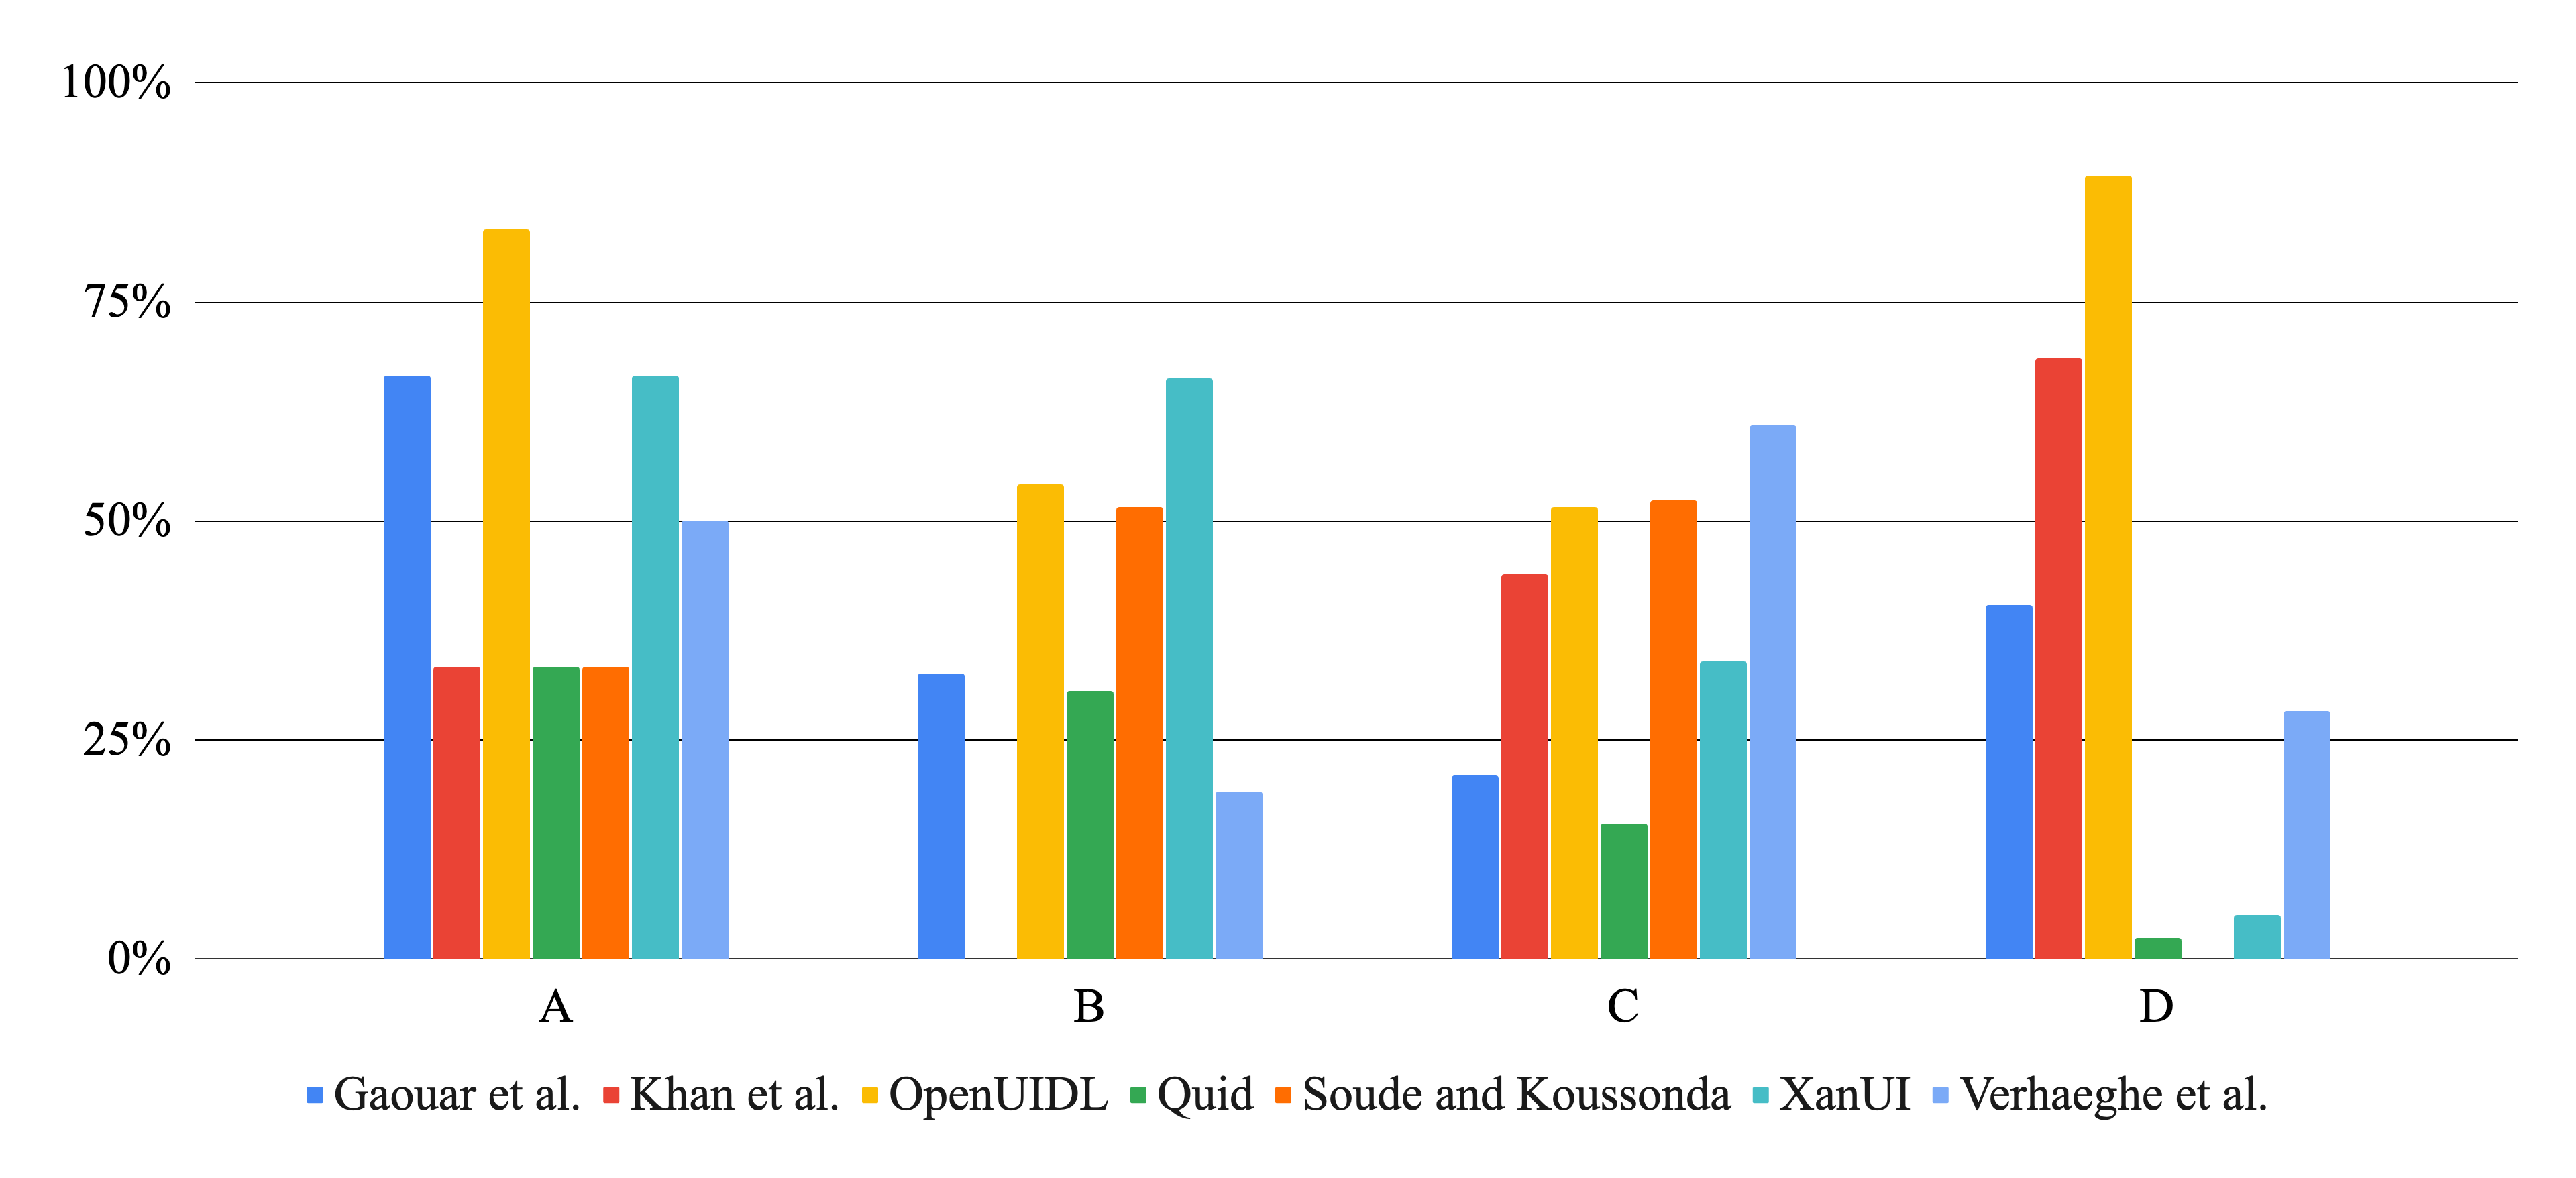
\includegraphics[width=\textwidth]{4-results-and-discussion/results-per-section}
    \caption{Results of the evaluation, presented per section}
    \label{fig:4-2-results-per-section}
\end{figure}

\begin{figure}
    \centering
    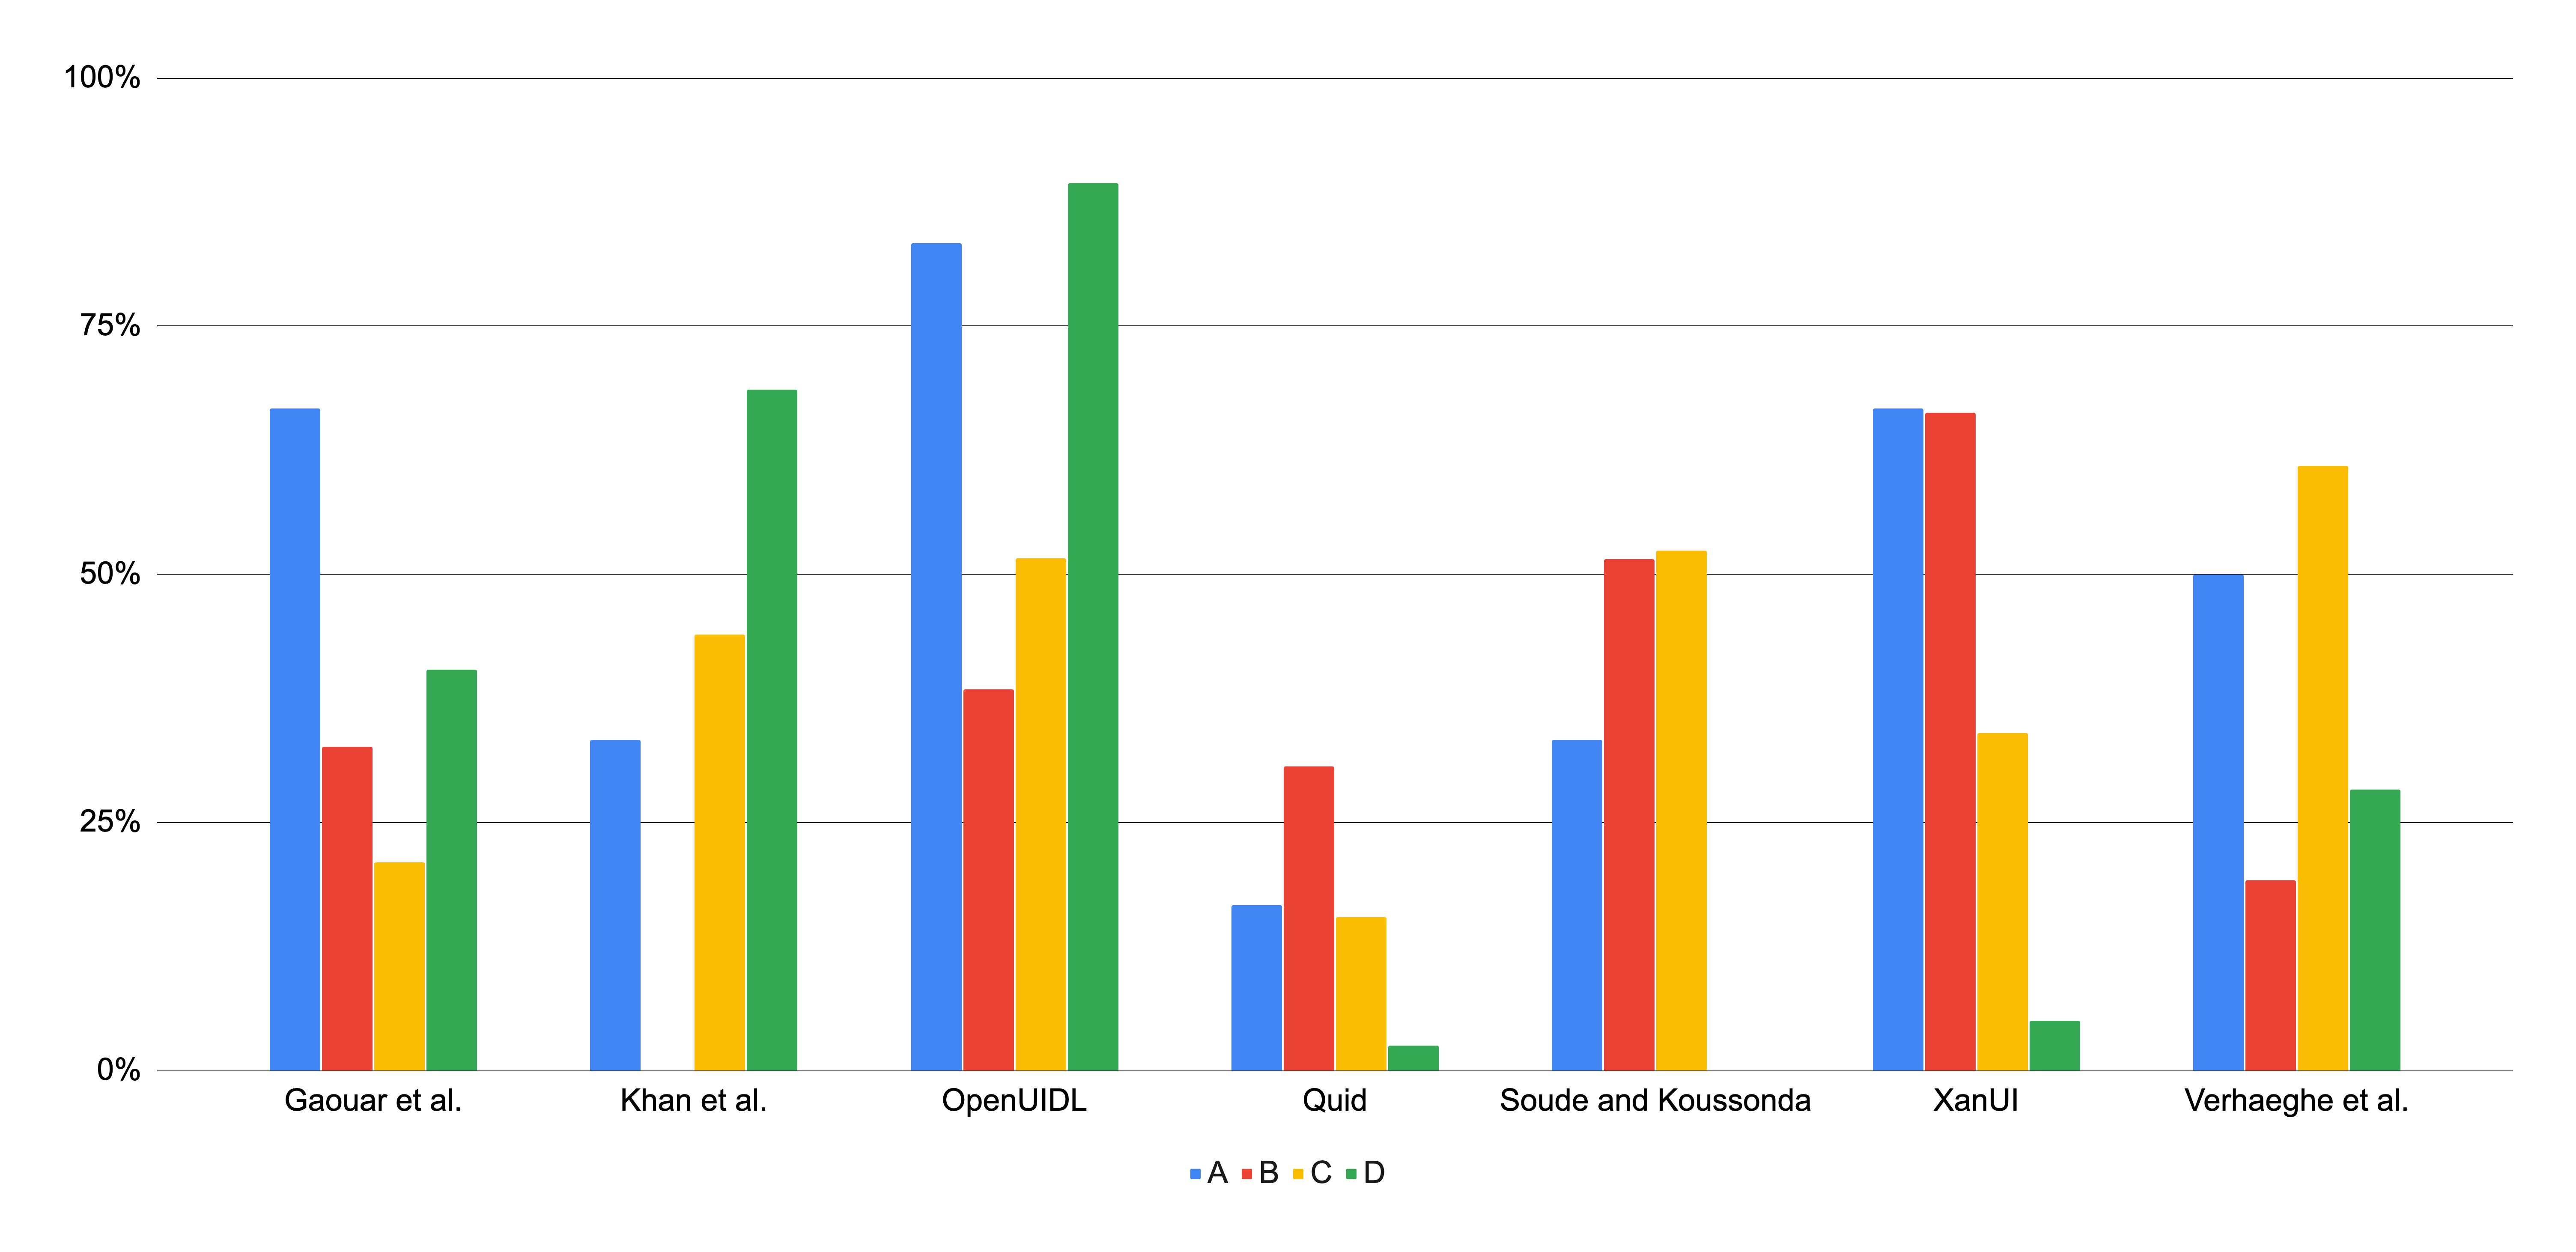
\includegraphics[width=\textwidth]{4-results-and-discussion/results-per-representation}
    \caption{Results of the evaluation, presented per representation}
    \label{fig:4-2-results-per-representation}
\end{figure}

\begin{figure}
    \centering
    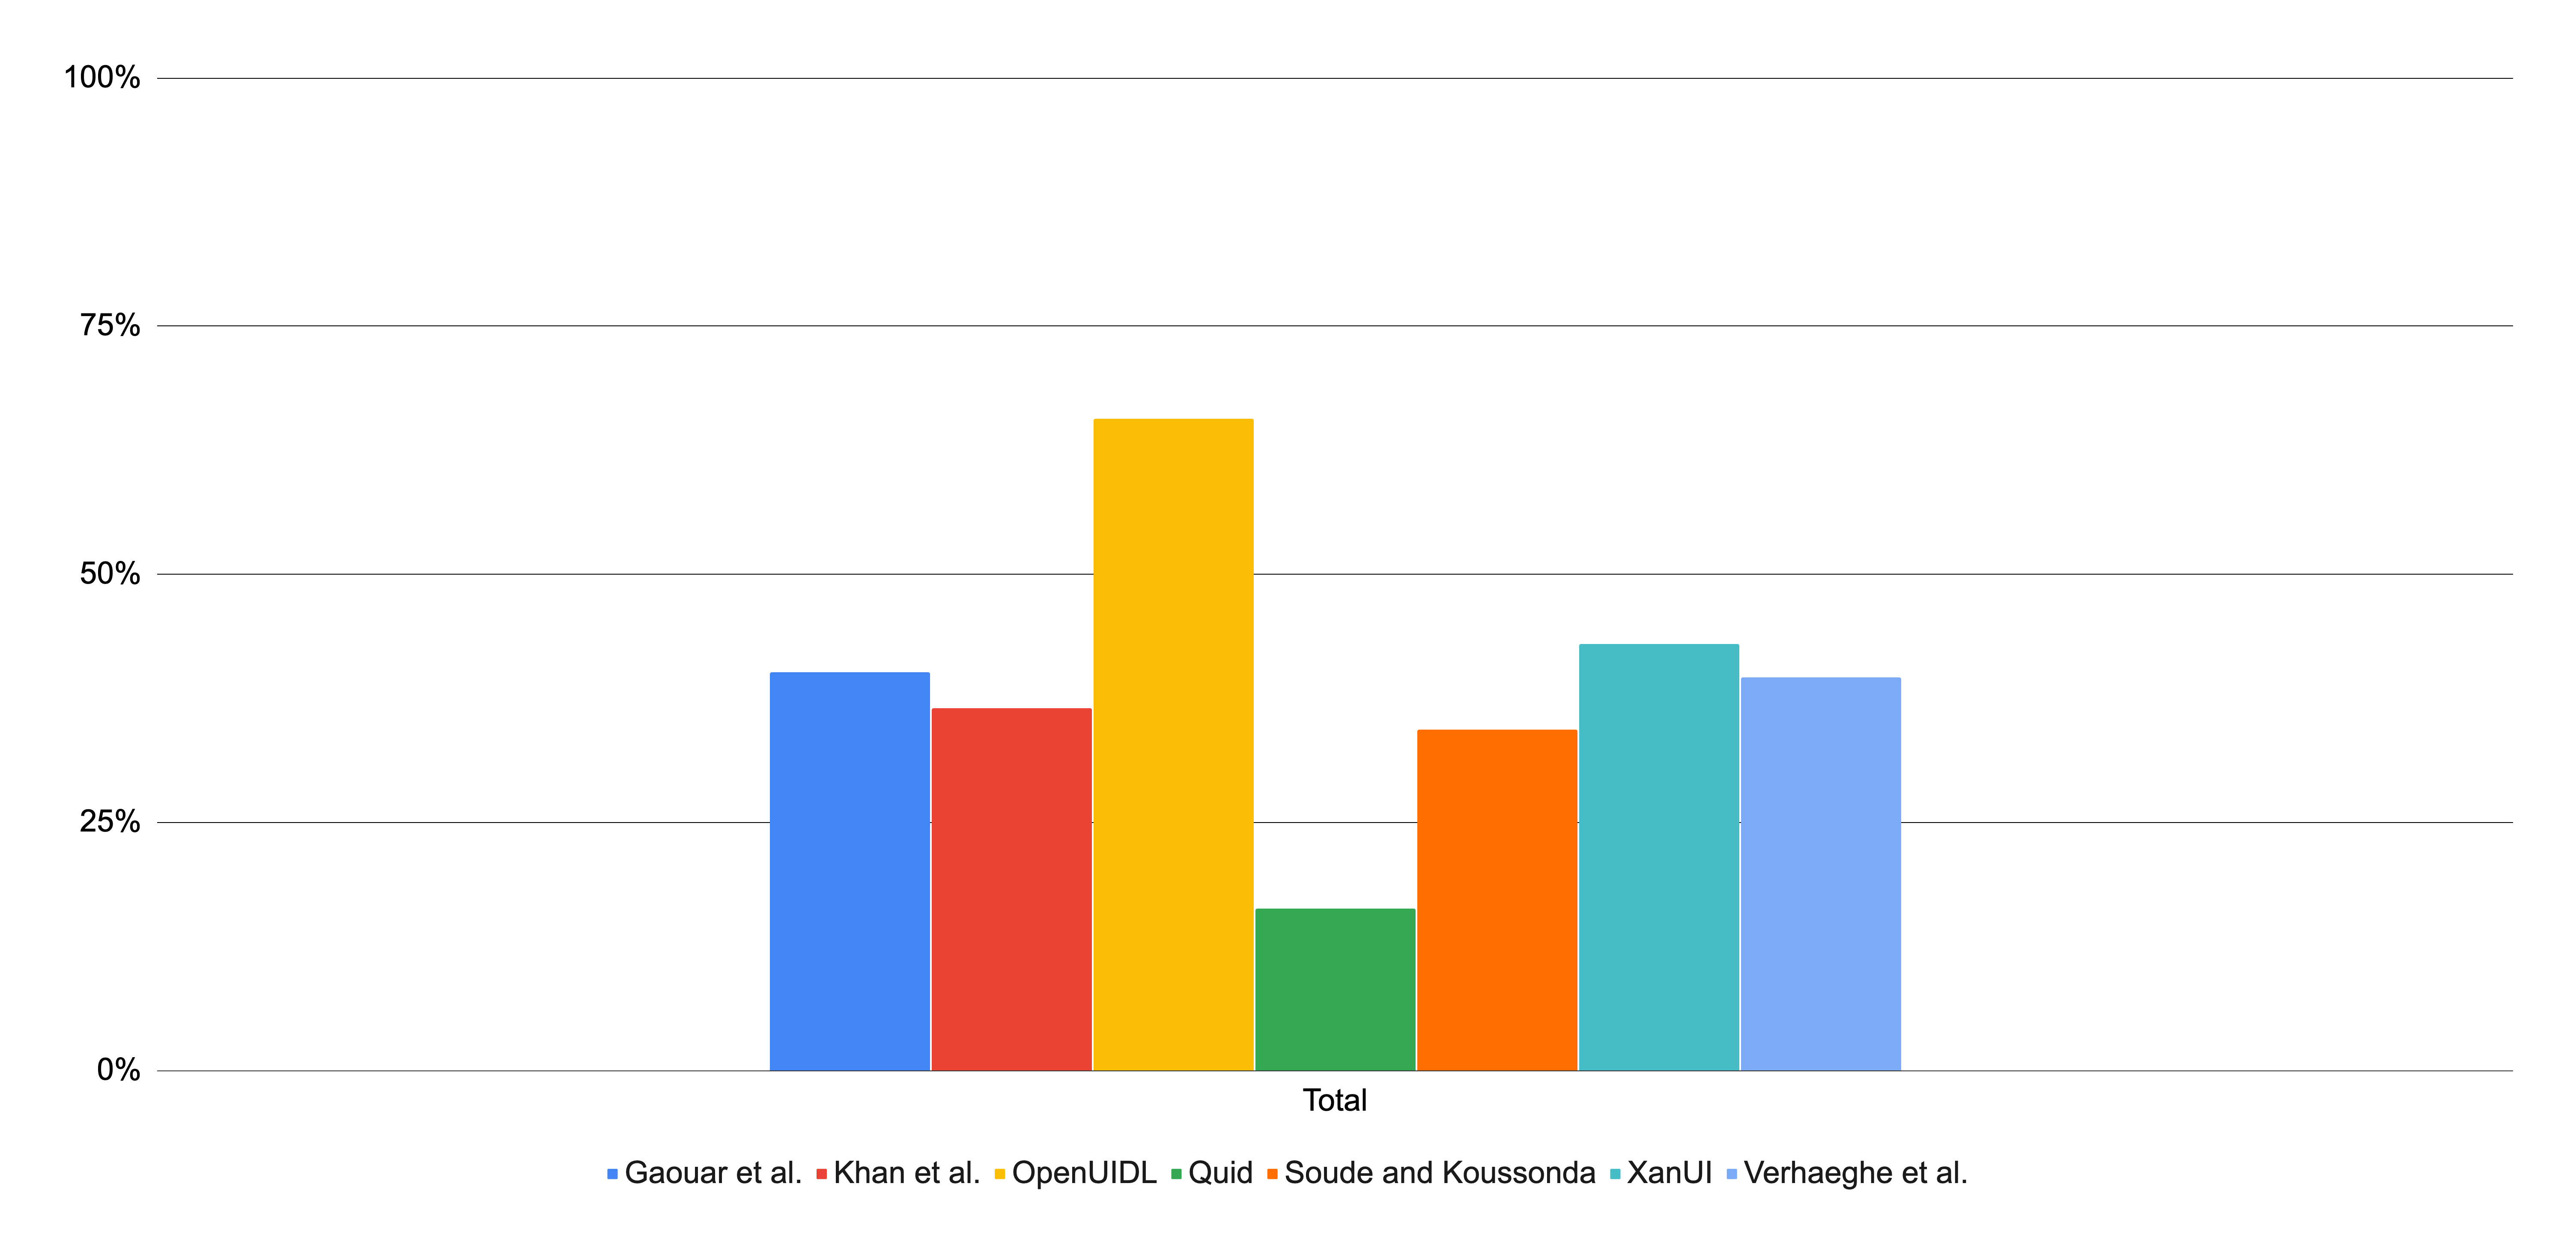
\includegraphics[width=\textwidth]{4-results-and-discussion/results-total}
    \caption{Overall results of the evaluation}
    \label{fig:4-2-results-total}
\end{figure}

\subsection{Case study}
Conclusions:
\begin{itemize}
    \item main takeaway: the results are very similar to the theoretical criteria!
    \item Quid isn't very expressive \textendash\ it's barely possible to do anything
    \item OpenUIDL actually allows to do something \textendash\  it was possible to prototype and customize quite a bit; the only thing missing was state and logic management (even though some was already present in a very primitive form!)
\end{itemize}

It turned out like this:
Figure~\ref{fig:4-2-board-view} presents the board view, as implemented in the selected languages.
\begin{figure}
    \centering
    \begin{subfigure}[m]{0.6\textwidth}
        \centering
        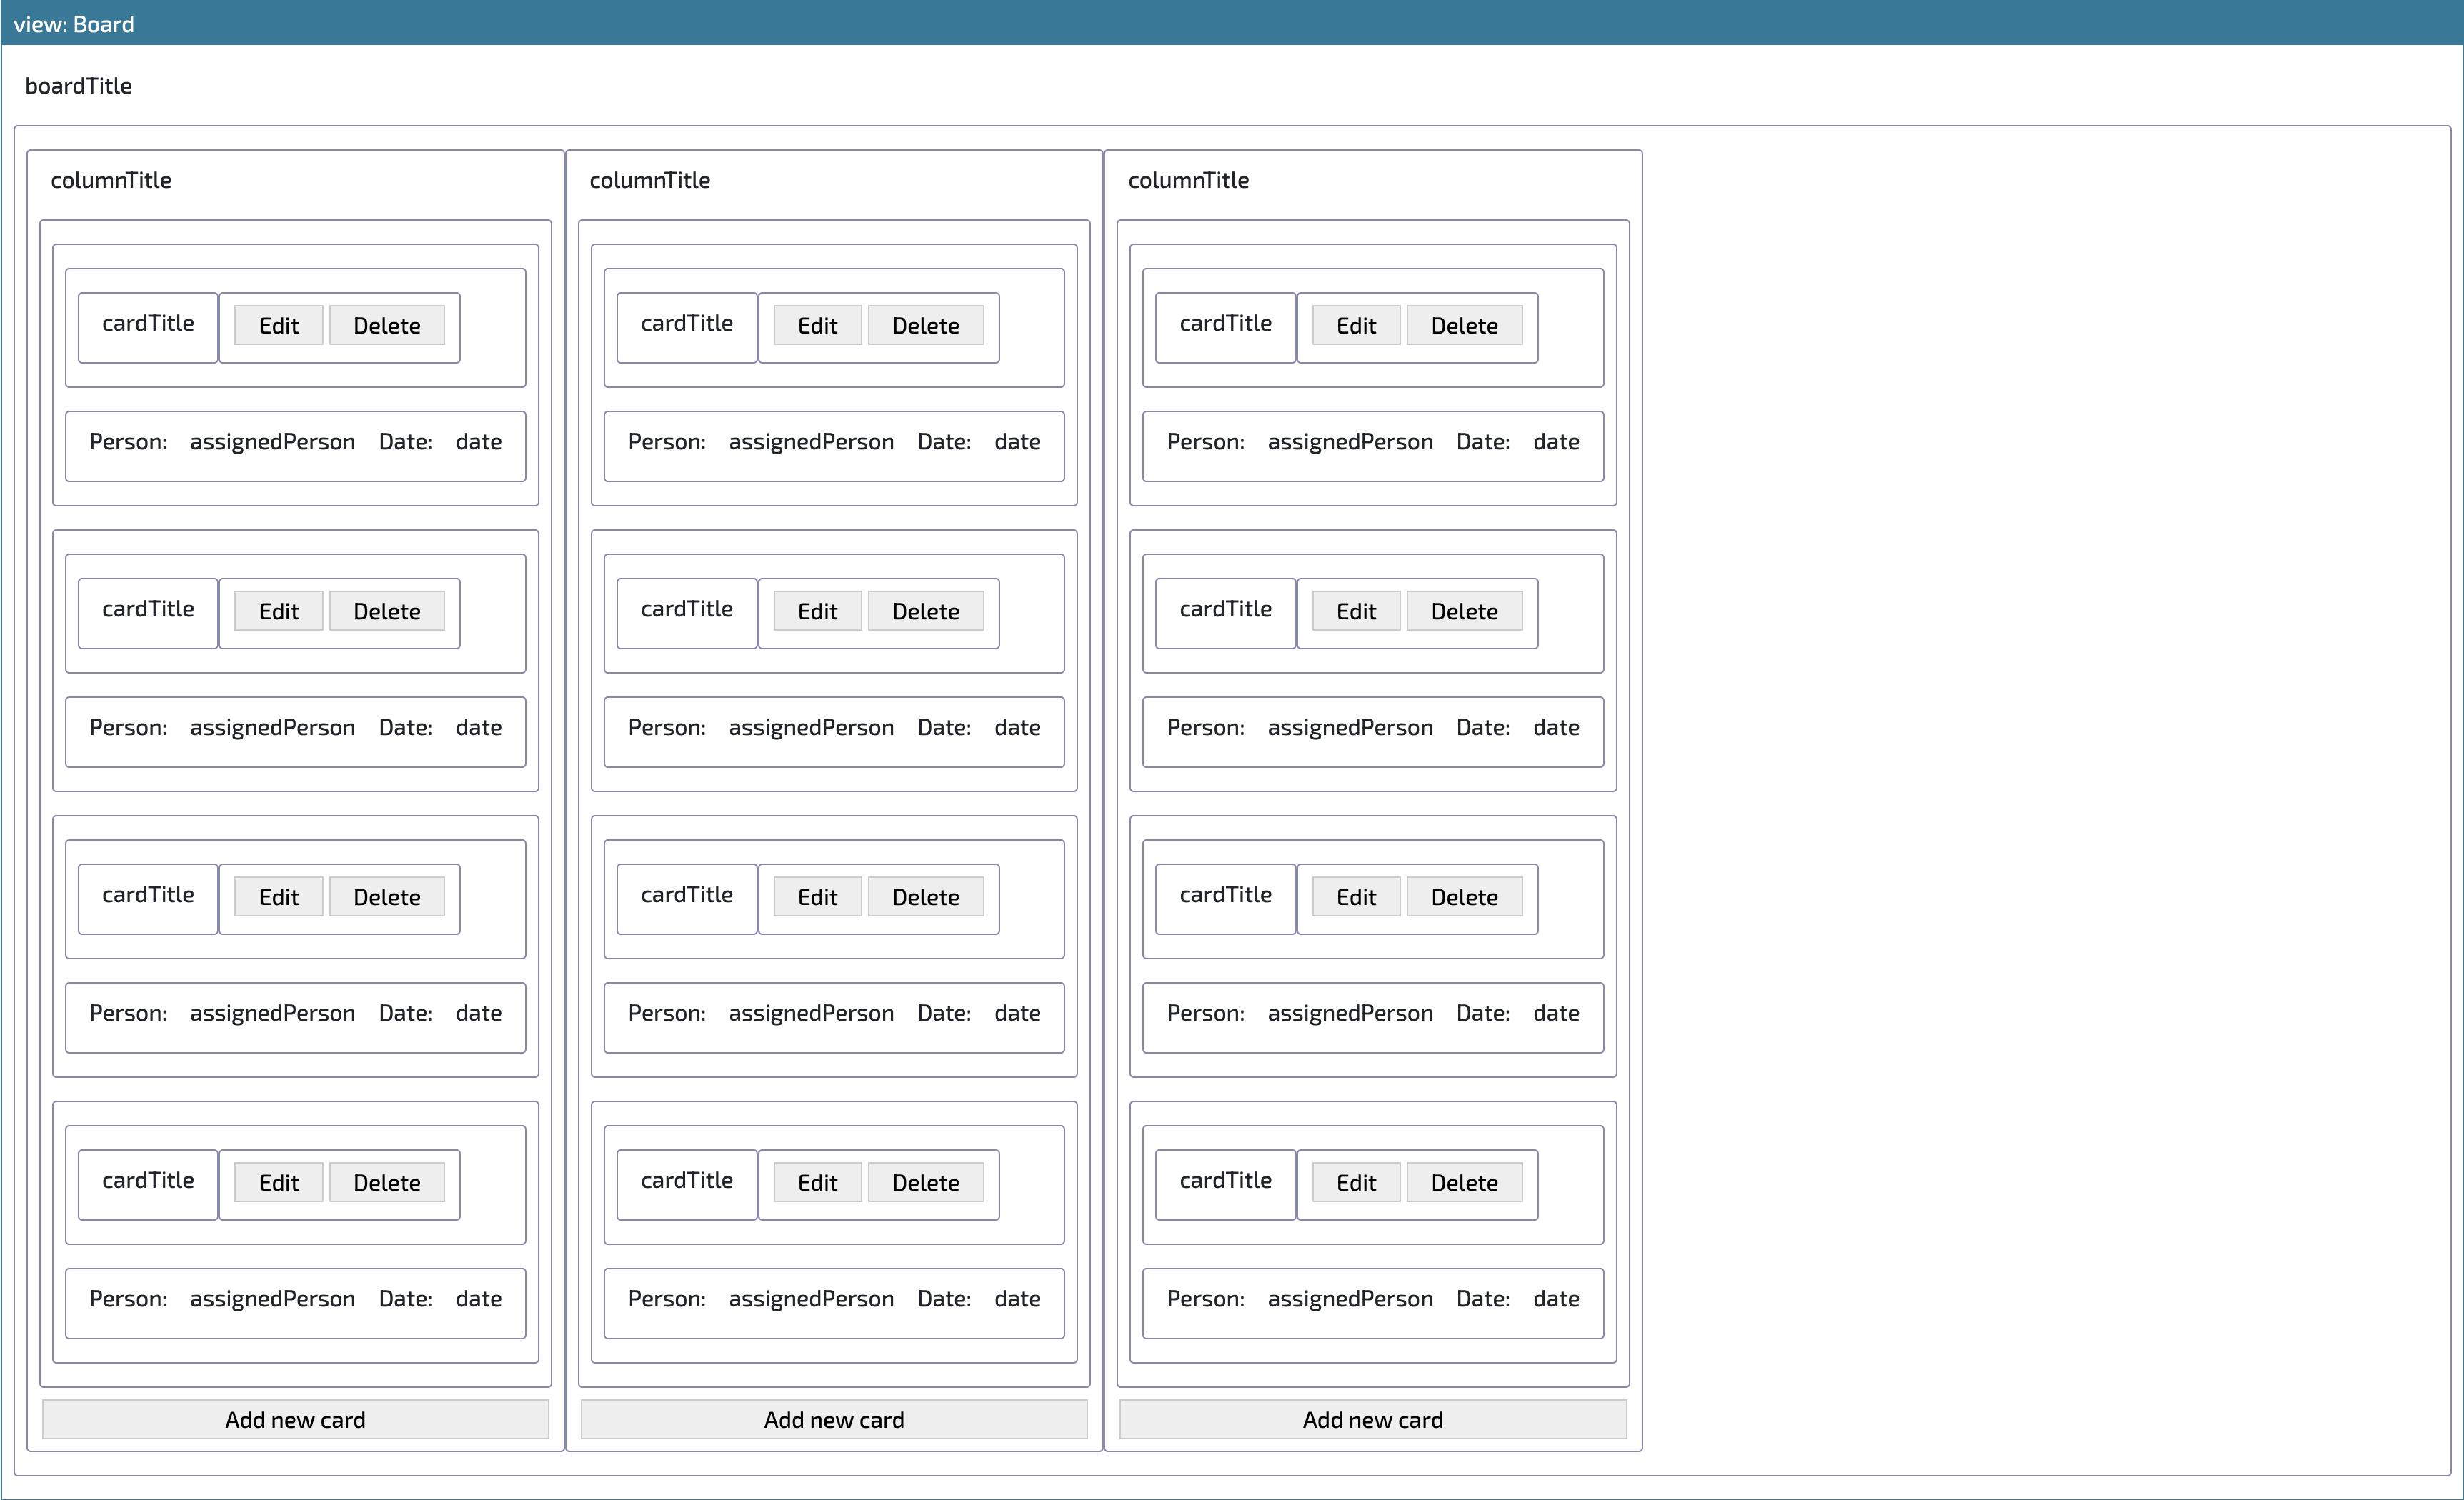
\includegraphics[height=0.25\textheight]{./4-results-and-discussion/quid-board-view}
        \caption{Board view implemented in Quid}
        \label{fig:4-2-quid-board-view}
    \end{subfigure}
    \hfill
    \begin{subfigure}[m]{0.35\textwidth}
        \centering
        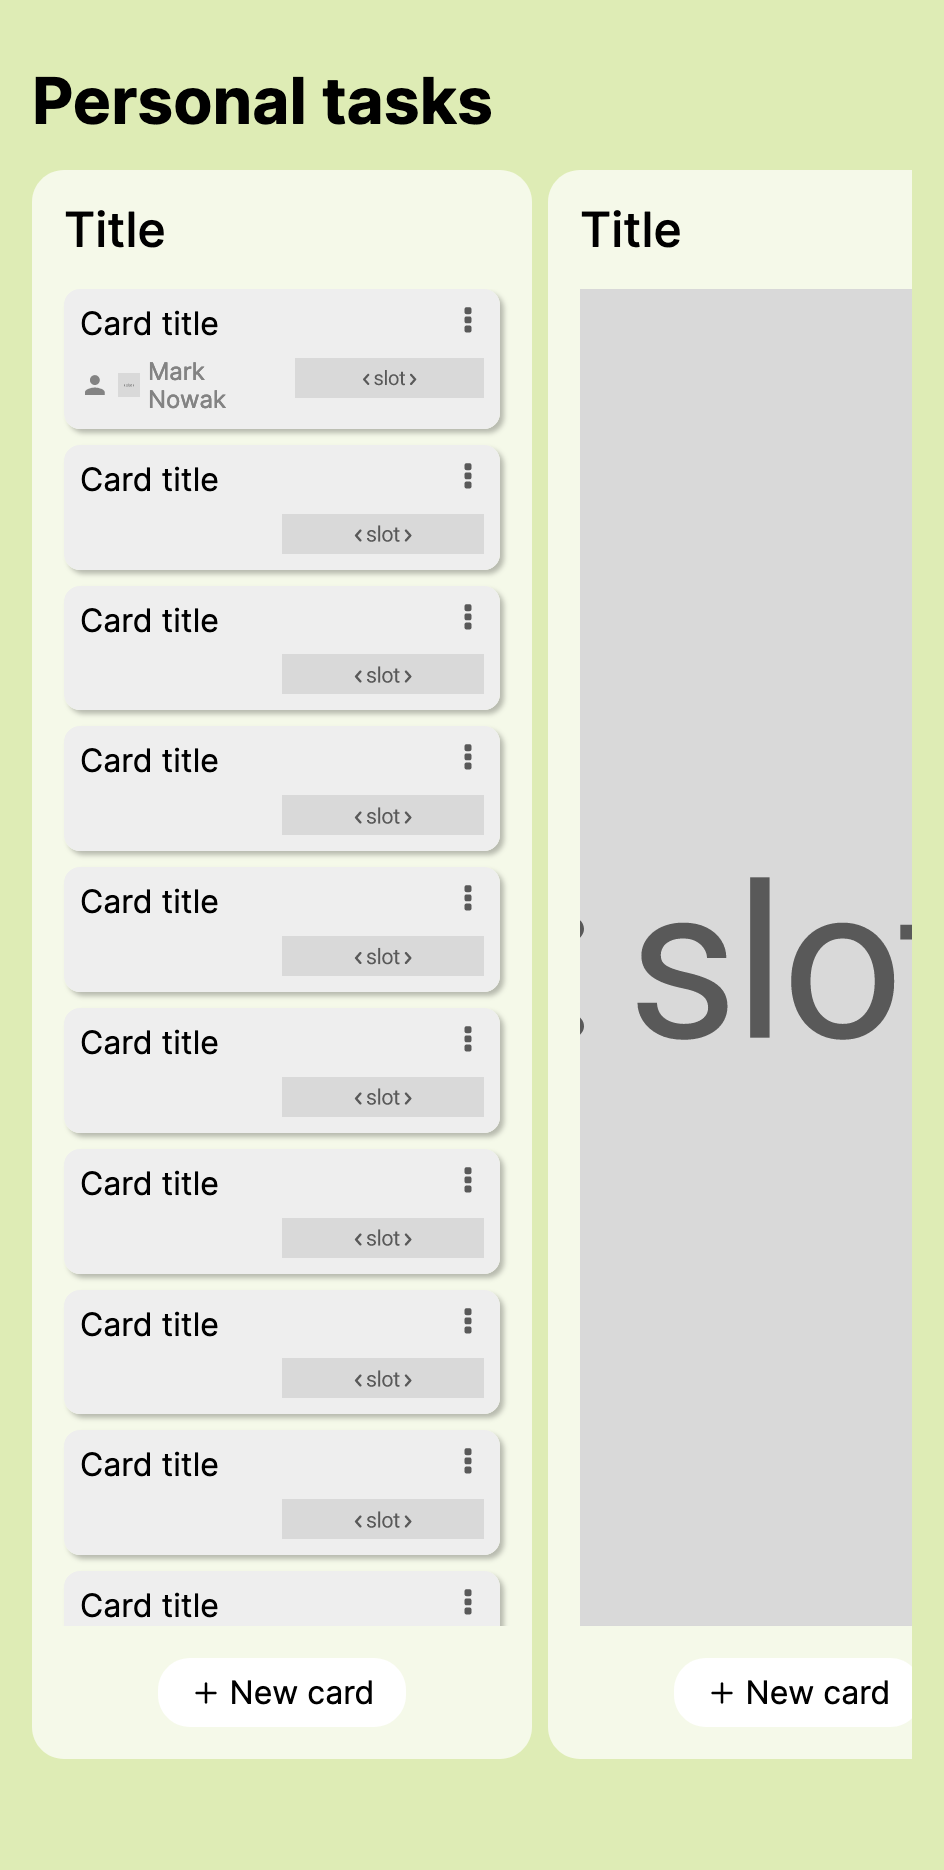
\includegraphics[height=0.4\textheight]{./4-results-and-discussion/openuidl-board-view}
        \caption{Board view implemented in OpenUIDL}
        \label{fig:4-2-openuidl-board-view}
    \end{subfigure}
    \caption{Implementations of the board view from the case study}
    \label{fig:4-2-board-view}
\end{figure}

\subsection{Results of the qualitative evaluation}\label{subsec:results-of-the-qualitative-evaluation}

Some initial thoughts:
Quid
\begin{itemize}
    \item the initial idea is great - the minimal language, the live preview
    \item the execution is lacking
    \item currently, the solution could be only viewed as a proof of concept, but nothing productive (not version 1.0 yet), the project doesn't seem maintained
    \item the documentation is too short and not detailed
\end{itemize}

OpenUIDL:
\begin{itemize}
    \item OpenUIDL looks like a relatively mature (and commercialized) solution, is well integrated with other solutions (deploying to some CDNs, integration with GitHub, etc.)
    \item there seems a lot of potential, but the capabilities for logic seem underdeveloped and can only be used to create simple, static pages
    \item the language is hidden behind an editor UI which is a good idea, because it could be difficult to write big projects
    \item in this way, though, it's impossible to use the language directly
    \item that the UI is a little buggy
\end{itemize}
